\newpage
\chapter{Machine Learning And Data Science}

Machine Learning is an area of computer science which focuses on making accurate 
predictions based on already gathered data and mathematical models.

\section{Core Concepts}

\begin{itemize}

    \item Historical Data: Refers to the data on which we are going to base our model. 

    \item Feature/Predictor vector \(X\): This some vector whose components represent the different numeric values of the characteristics 
    of some object.

    \item Function \(f\): is called \emph{target function} \(f: \mathcal{X} \to \mathcal{Y}\) which makes a perfect approximation 

    \item Label \(y\): Is some image of one \(x \in \mathcal{X}\) 

    \item Data Sample \(D\): this is a set of pairs \((x_i, y_i)\)

\end{itemize}

Our goal is to find a function \(g: \mathcal{X} \to \mathcal{Y}\) which approximates \(f\)

\subsection{Solution Strategy}

\begin{itemize}

    \item The learning algorithm \(\mathcal{A}\) uses data to select, from a set of candidate functions, the function \( g \) that best approximates the target function \(f\).

    \item \( \mathcal{H} \): Set of candidate functions (hypothesis set). (Example: linear functions)

    \item \( g \in mathcal{H} \) is also called the \emph{final hypothesis}, which the algorithm selects at the end.

\end{itemize}

\section{Central Learning Problems in Machine Learning}

\textbf{Supervised Learning}

\begin{itemize}

    \item Sought: Unknown target function.

    \item Data: Input--output pairs.

    \item Approximate the unknown target function \( f_{\text{target}} \) with a hypothesis \( h \) such that \( h \approx f_{\text{target}} \).

\end{itemize}

\textbf{Unsupervised Learning} 

\begin{itemize}
   
    \item Sought: Unknown function that describes the data.

    \item Data: Only input data (no labels).

    \item Find a function \( f \) that describes the structure or distribution of the data well. 
     
\end{itemize}

\textbf{Reinforcement Learning}

\begin{itemize}
    
    \item Sought: Unknown strategy \( S \) that maximizes a reward.
    
    \item Data: (1) Input  (2) Possible output (3) Evaluation of output (reward).
    
    \item Find a function \( f \) that approximates the optimal strategy \( S^* \) that maximizes the expected reward.

\end{itemize}

\section{Data Preparation}

The data set \(\mathcal{D}\) we be spit into training and test data to minimize our 
margin of error. If a model is trained only used the same data again, and again it will become 
less reliable with new data which differs from its training set. Making out of sample errors 
difficult to spot.

For mitigating this problem as well as to make our data suitable for training a model we use both splitting the data set into 
training and validation data, and another is to scale data, eliminate NaN values and in general data cleaning.

Another way of improving the quality of the data set is to add a certain degree of noise to our sample data. Thus, 
converting \(y\) into a probability-variable dependent on \(x\). Therefore, \(f \to P(y \mid x)\).

\section{Feature Scaling}

\emph{Feature scaling} is a technique used to standardize the range of independent variables or features or predictors of data.
In machine learning, it is crucial because many algorithms are sensitive to the scale of the input data.

Common methods for feature scaling include:

\begin{itemize}
    
    \item \emph{Min-Max Scaling (Normalization)}: This technique scales the data to a fixed range, usually 0 to 1. The formula is:
    
    \[
        X' = \frac{X - X_{min}}{X_{max} - X_{min}}
    \]

    By adding \((b - a)\) to the formula we can scale it to any range \([a, b]\):

    \[
        X' = a + \frac{(X - X_{min})(b - a)}{X_{max} - X_{min}}
    \]

    \item \emph{Standardization (Z-score Normalization)}: This method transforms the data to have a mean of 0 and a standard deviation of 1. The formula is:
    
    \[
        Z = \frac{X - \mu}{\sigma}
    \]

    where \(\mu\) is the mean and \(\sigma\) is the standard deviation of the feature.

    \item \emph{Robust Scaling}: This method uses the median and the interquartile range (IQR) for scaling, making it robust to outliers. The formula is:
    
    \[
        X' = \frac{X - \text{median}}{\text{IQR}}
    \]

\end{itemize}

\section{Hyper Parameters}

A \emph{hyper-parameter} is a parameter used by a model/algorithm which can not be approximated directly during the training process.
For example the \(k\) by K-Means is given at the start.

\subsection{Hyper-parameter Tunning}

\emph{Hyper-parameter tunning} is the process of improving the hyper-parameters via validations methods. In such methods not only is model 
tested against other models with the same hyper-parameters, but also against the same model with different hyper-parameters.

\section{Accuracy Metric For Regression}

\subsection{R-squared}

\emph{R-squared} provides a measurement of how much variation in the response does the model explain.

\[
    R^2 = \frac{\var(\text{fitted})}{\var(\text{response})}, \quad 0 \le R^2 \le 1
\]

with 

\[
    \var(\text{response}) = \var(\text{fitted}) + \var(\text{residuals})
\]

This metric is not available for all models. Linear regressions among other support this metric.

A problem of this metric is that it increases when more predictors are added which means that even not relevant coefficients are 
taking into consideration.

\subsection{Adjusted R-squared}

This is a penalized version \(R^2\) to avoid taking irrelevant predictors.

\[
    \text{adjusted }R^2 = 1 - (1 - R^2) \frac{N - 1}{N - p} 
\]

with \(N\) as the sample size and \(p\) as the number of coefficients in out linear model.

\subsection{Mean Squared Error}

This is the classical function for our linear regression

\[
    \mathrm{MSE} = \sum_{i = 1}^{N} (y_i - \tilde{y_i})^2
\]

\section{Validation}

\emph{Validation} refers to process of evaluating our algorithms and models based on specific parameters 
and procedures. 

The hypothesis gained from a model which is going to be validated is marked as \(\overline{g_n}\). 

The types of data which arise from the splitting of the data are 

\begin{itemize}

    \item \emph{Training Data}: Data used for training the model. 

    \item \emph{Validation Data}: Used for testing our model against other models in situations like hyper-parameter tunning.

    \item \emph{Test Data}: Used to test the accuracy of the model at predicting, knowing the labels.

\end{itemize}

\subsubsection*{Quote from the statistical Learn-theory}

The more often you use a data-set for training a model, taking decisions, etc. The hard is to approximate 
the capacity of the data-set to approximate the out-of-sample error. 

\subsection{Hold-Out-Validation}

Data points are randomly shuffled into training and test data. 

\subsection{Cross Validation}

\emph{Cross Validation} is a technique to improve a models accuracy by presenting training the model on different splits on the data. 
It can also help us compare different algorithms on the splits and then choose the model with best general accuracy.

The procedure consists on splitting the data-set into \(V\) different sub-sets of equal size called \emph{folds}. Then, we train our model \(V\)-times, each time using \(V-1\) disjoint sub-sets for 
training and the remaining one for testing. The final out-of-sample error is given by the average of all the out-of-sample errors gotten from each iteration.

The nomenclature:

\begin{itemize}
    
    \item \emph{Number of data points in the training set} \(N_{\text{train}} = \frac{V - 1}{V} N\)

    \item \emph{Number of data points in the validation set} \(N_{\text{val}} = \frac{1}{V} N\)

    \item \(e_n:= E_{\text{val}} (\overline{g_n}) = e(\overline{g_n}(x_n), y_n)\)

    \item \emph{Cross Validation Error} \(E_{\text{V-fold CV}} = \frac{1}{V} \sum_{n = 1}^{V} E_v\)

\end{itemize}

One more use case of cross validation is to estimate \emph{tunning/hyper-parameter}, which are not directly optimized by  the model, but determined by the person 
performing the analysis.

\subsection{Leave One Out Cross Validation}

\emph{Leave One Out Cross Validation} work by leaving always \textbf{one data point out}, instead of a fold.
This is the same as a \(N\)-fold cross validation.

The nomenclature:

\begin{itemize}
    
    \item \(e_n:= E_{\text{val}} (\overline{g_n}) = e(\overline{g_n}(x_n), y_n)\)

    \item \emph{Cross Validation Error} \(E_{\text{CV}} \frac{1}{N} \sum_{n = 1}^{N} e_n\)

\end{itemize}

\subsection{Confusion Matrix}

A \emph{confusion matrix} is a table that is often used to describe the performance of a classification model (or "classifier") on a set of test data for 
which the true values are known. It allows the visualization of the performance of an algorithm. 

For example, in a binary classification problem, the confusion matrix is a 2x2 table that summarizes the counts of true positive \(TP\), 
true negative \(TN\), false positive \(FP\), and false negative \(FN\) predictions made by the model. 

\subsection{Sensitivity and Specificity}

\emph{Sensitivity} measures the proportion of actual positives in the data that are correctly identified as such (true positive rate). It is calculated as:

\[
    \text{Sensitivity} = \frac{TP}{TP + FN}
\]

The denominator represents the sum of the column corresponding to actual positive cases, while the numerator represents the true positive cases.

\emph{Specificity} measures the proportion of actual negatives in the data that are correctly identified as such (true negative rate). It is calculated as:

\[
    \text{Specificity} = \frac{TN}{TN + FP}
\]

The numerator is the sum of all cells which are not in row or column of positive cases, while the denominator is the sum of the row corresponding to actual negative cases plus 
our previous numerator.

\section{Learning Principles}

\subsection*{Ockham}

The simplest model which approximates the data is also the more plausible. 

\subsection*{Corrupted Samples}

If the sample are corrupted, biased or contains errors then the model will also not be neutral 
and will give false approximations.

\subsection*{Data Snooping}

If a data-set affects the learning process then its capacity of approximating the out-of-sample error 
was reduced. 

\section{Feature Selection}

This is the process of choosing the "right" features to use in a model. This can be done manually using statistical 
testing, examining correlation, and domain knowledge or automatically via algorithms.

The automatic variant do deliver accurate models on the paper, but they may not reflect the reality of the function we are trying to 
approximate or they do not take certain relationships in the data. For these reasons, regularization methods are mostly preferred, but feature 
selection is still useful if done correctly.

\subsection{Best Subset Selection}

\emph{Best subset selection} consist on testing all \(2^p\) possibilities of combining \(p\) features and then perform cross validation 
with all possibilities to get the best features. 

This is obviously very expensive.

\subsection{Forward Stepwise Selection}

Adding variables one at a time, choosing a variable which delivers the best result.

\subsection{Backward Stepwise Selection}

Removing variables one at a time, choosing the variable the one which contributes the least to the error function.

\section{Regularization}

\emph{Regularization} is the process of making the algorithm less sensible to data out of the sample our in other words,
helps the learning algorithm to minimize the output-of-sample error. This is accomplished by different methods like adding error terms, 
special procedures etc.

In general, with regularization we want to decrease the complexity of our approximations to the target function to minimize overfitting.
with

We define 

\[
    \beta_i = \sum_{i = 1}^{k} w_i
\]

as the sum of coefficient of our parameter vector \(w \in \R^k\).

\subsection{Ridge Regression}

This is a regularization technique used  specially in linear models to prevent overfitting by discouraging the model from assigning 
excessively large values to its parameters.

\[
   \mathrm{Ridge}: h(x_i)  + \lambda \sum_{i = 1}^{p} \beta_i^2
\]

\textbf{Example:}

This example uses linear regression. Therefore, 

\begin{align*}
    E_{\text{in}}(h) &= \frac{1}{N} \sum_{n = 1}^{N}(h(\phi(x_n)) - y_n)^2 \\
    E_{\text{in}}(h) &= \frac{1}{N} \sum_{n = 1}^{N}(w^Tz_n - y_n)^2 \\
    E_{\text{in}}(h) &= \frac{1}{N} (Zw - y_n)^T(Zw - y)
\end{align*}

And 

\[
    Z := \begin{bmatrix}
        z_1^T \\ z_2^T \\ \vdots \\ z_{n}^T 
    \end{bmatrix}
\]

Our augmented error is given by 

\begin{align*} 
    E_{\text{aug}} (w) &= E_{\text{in}} + \frac{\lambda}{N} w^T w \\ 
    &= \frac{1}{N} (Zw - y_n)^T(Zw - y) + \frac{\lambda}{N} w^T w 
\end{align*}

To minimize it we want to set its gradient to 0 which gives us  

\begin{align*}
    \nabla_w E_{\text{aug}}(w) = 0 \implies & Z^T(Zw - y) + \lambda w = 0 \\
    & Z^TZw - Z^Ty + \lambda w = 0 \\
    & (Z^TZ - Z^T I)w + Z^T y= 0 \\
    & w_{\text{reg}} = (Z^T Z + \lambda I)^{-1} Z^T y 
\end{align*}

Finally, as a remainder the formula without regularization

\[
    w_{\text{lin}} = (Z^T Z)^{-1} Z^T y
\]

\subsection{LASSO Regression}

This is similar to Ridge regression in the sense that we are adding a penalty term times \(\lambda\) at the end of our optimization problem, but 
instead of summing the square ..., we add the absolute value

\[
   \mathrm{LASSO}: h(x_i)  + \lambda \sum_{i = 1}^{p} | \beta_i |
\]

It is important to note that both this and Ridge regularization is very sensible to the scaling of our features.

\section{Errors}

\subsection{In Sample Errors}

The \emph{in-sample-error} is the mean of the amount of samples which were incorrectly labeled. 

\[
    E_{in} (h) = \frac{1}{N} \sum_{i = 1}^{N} W(h(x_i) \neq f(x_i))
\]

where

\[
    W(Expr) = \begin{cases}
        1 & Expr = True \\ 
        0 & Expr = False
    \end{cases}
\]

It is the median of the errors made on the training data. 

\subsection{Out of Sample Errors}

This refers to all errors which can occur due to the lack of data. Obviously we do not 
have all possible samples which will exists.

\[
    E_{out} (h) = P[h(x) \neq f(x)]
\]

These errors have a randomness factor, or in other words an unknown probability distribution.
They are harder to calculate due to their nature. 

\section{Approximation and Generalization}

When trying to approximate the target function \(f\) we encounter the problem that our data may not 
give us the exact function because of the lack of data. To want to minimize the in-sample error 
but also make out approximation as general as possible.

\emph{Approximation:} Small in-sample-error

\emph{Generalization:} \(E_{\text{out}} \approx E_{\text{in}}\)

\subsection{Bias and Variance}

Fitting the training data well, but making poor predictions, is called the \emph{bias-variance} trade-off.

The \emph{bias} is a measurement of the difference between all the possible data predicted via our final 
hypothesis \(g\) the target function \(f\). In other words, how much our approximations deviates from the actual perfect 
prediction.

The \emph{variance} measures how much a final hypothesis \(g\) gotten from one specific 
data-set differ from one another.

There are two extreme cases: one is when the hypothesis-set has only one function, therefore we have zero 
variance and a big bias; and the other case is when the set is large and different data-sets produce similar functions, 
therefore we get a near zero bias but a high variance.

With this in mind we now define 

\[
    E_{\text{out}} = \text{ Bias } + \text{ Variance} 
\]

\textbf{Example:}

Our target is \(\sin(\pi x)\), and our hypothesis-sets are \(\mathcal{H}_0\) the set of all horizontal 
lines \(h(x) = b\) and \(\mathcal{H}_1\) the set of all lines \(h(x) ax + b\). The training-sets are two data-points of the internal 
\([-1,+1]\).

\subsection{Learning Curves}

\emph{Learning curves} plot \(E_{\text{in}}\) and \(E_{\text{out}}\) depending on the number of the 
data-points.

\subsection{Overfitting}

\emph{Overfitting} refers to the situation when a model adapts itself too much to a given data-set. Precisely, it is the process 
in which hypotheses \(h\) continuously reduce the in-sample error, but leading to a bigger output-of-sample error.

We define \emph{overfitting} for a hypothesis \(h\), if for another hypothesis \(h'\) the following is true 

\[
    E_{\text{in}}(h) < E_{\text{in}}(h') \text{ but } E_{\text{out}}(h) > E_{\text{out}}(h')
\]

In summary, noise in the data (stochastic or deterministic) have a negative effect on the learning process and can lead 
to overfitting. To address this problem we will use \emph{regularization}.

\subsection{Underfitting}

\emph{Underfitting} refers to the case when the model has not been trained with enough data to make 
accurate approximations.

\subsection{The Augmented Error}

We define the \emph{augmented error} as 

\[
    E_{\text{aug}}(w) = E_{\text{in}}(w) + \frac{\lambda}{N}w^T w 
\]

\(\lambda\) is the parameter for how much we should regularize, \(w^T w\) is the punish-term based on the weight of the vector and 
\(N\) is the number of data points.

\section{Classification And Regression}

\emph{Classification} predicts categories based on discrete labels i.e classes or groups, while \emph{regression} predicts 
on continuous values i.e. identifying trends and patterns.

Common classification functions with example models: 

\begin{itemize}
   
    \item Binary cross entropy in logistic regression, ironically.

    \item Categorical cross entropy. 

    \item Hinge loss for support vector machines.

\end{itemize}

Common regression functions with example models: 

\begin{itemize}
   
    \item Mean square error in logistic regression. 

    \item Information gain in  decision tree regressors.

\end{itemize}

\section{The Perceptron} 

\emph{The perceptron} is our first model in machine learning. It consists on having a separate vector \(w \in \R^d\) which consist of weights which are going to be 
associated with the components of \(x \in \mathbb{R}^d\). We also define \(y \in \{-1,1\}\),  and some value \(b\) to work as our border between the categories of y. 
We classify our prediction based on the result 

\[
    \sum_{i = 1}^{d} w_i x_i > b \text{ accept }
\]

\[
    \sum_{i = 1}^{d} w_i x_i < b \text{ reject }
\]

More precisely 

\begin{align*}
    \sum_{i = 1}^{d} w_i x_i + 1 \cdot b &> 0 \\ 
    \sum_{i = 1}^{d} w_i x_i + x_0 \cdot w_0 &> 0  \mid x_0 = 1 \quad w_0 = b\\
    \sum_{i = 0}^{d} w_i x_i &> 0  \\
    w^T x &> 0 
\end{align*}

Finally, to get our respective \(y\) we define the following function 

\[
    \text{sign}(w^T x) = \begin{cases}
     1, &\sum_{i = 1}^{d} w_i x_i > 0\\
    -1, &\sum_{i = 1}^{d} w_i x_i < 0
    \end{cases}
\]

And we get our final perceptron equation 

\[
    h(x) = \text{sign}(w^Tx)
\]

For the case \(d = 2\),  our vector \(w\) defines a \emph{line}. 

\begin{align*}
    w_0 \cdot 1 + w_1 x_1 + w_2, x_2 &= 0 \\ 
    x_2 &= - \frac{w_1}{w_2} x_1 - \frac{w_0}{w2} \\ 
    x_2 &= m x_1 + c
\end{align*}

Here a visualization 

\begin{center}
\begin{tikzpicture}[>=Stealth, scale=1.2]

% Axes
\draw[->] (-0.5,0) -- (4.5,0) node[right] {$x_1$};
\draw[->] (0,-0.5) -- (0,4.5) node[above] {$x_2$};

% Positive class (blue)
\foreach \x/\y in {3/3.5, 3.6/3.1, 2.7/2.8, 3.2/2.5, 2.5/3.2}
    \fill[blue] (\x,\y) circle (3pt);

% Negative class (red)
\foreach \x/\y in {0.6/0.8, 1.1/0.4, 0.4/1.2, 1.4/1.1, 0.8/1.5}
    \fill[red] (\x,\y) rectangle +(6pt,6pt);

% Decision boundary line (example)
\draw[thick] (0.2,4) -- (4,0.3);
\node at (4.1,1.8) {$w_1 x_1 + w_2 x_2 + 1 \cdot b = 0$};

\end{tikzpicture}
\end{center}

Note that \(y\) is not used for the visualization, as it is just using in the \(\text{sign}\) function to as for the classification. 

\section{The Perceptron Learning Algorithm}

The \emph{PLA} modifies \(w\) until the data are linearly separated, as long it is possible. 
It can be the case that in the current space it is not possible. Formally, if there exists a \(w^*\) such that 
\(h(x_i) = y_i, \forall (x_i, y_i) \in \mathcal{D}\).

It goes as follows: 

\begin{itemize}

    \item \emph{Data:} \((x_i, y_i)\) with \(x\) being a vector \(i = 1, \ldots, N\).
    
    \item \emph{Assumption:} The data are linearly separable, i.e., we can separate the data into their classes using a line (\(d = 2\)) or a hyperplane (\(d > 2\)).

\end{itemize}

Let \(t = 0, 1, 2, \ldots\) be the current iteration step, and let \(w^{(t)}\) denote the vector \(w\) at iteration step \(t\).  
Set \(t = 0\) and \(w^{(0)} = 0\).

\begin{enumerate}

    \item Use the perceptron with \(w^{(t)}\) and classify all data \(\mathbf{x_i}, i = 1, \ldots, N\). The labels predicted by the perceptron are denoted by \(y_{i,\text{pred}}\).
    
    \item Select any pair \((x_j, y_j)\) that was misclassified (i.e., \(y_{j,\text{pred}} \neq y_j\)), and denote it by \((x^{(t)}, y^{(t)})\). If no such pair exists, terminate.
    
    \item Update the weight vector \(w\) using the following rule:
    
        \[
            w^{(t+1)} = w^{(t)} + y^{(t)} x^{(t)}
        \]

        This just means taking the current \(w\) and adding the vector \(x\) times the corresponding label \(y\) which was expected.
         
    \item Increase \(t\) by 1 and return to step 1.
    
    \item After we got our final weights, we get our line or hyperplane by manipulating our 
    expression \(\sum_{i = 0}^d x_i w_i = 0\)

\end{enumerate}

\section{Pocket Algorithm}

The \emph{pocket algorithm} is an extension of the perceptron learning algorithm to handle non-linear separable data-sets. This 
achieved by setting a maximum number iterations while also keeping track of the vector with the lowest in-sample error value. 

\begin{enumerate}

    \item Initialize \( w \) and set \( w_{\text{best}} = w \).
    
    \item Compute the current in-sample error \( E_{\text{best}} = E_{\text{in}}(w) \).
    
    \item For each iteration:
    
     \begin{enumerate}
        
            \item If a point \( (x_i, y_i) \) is misclassified, update:
        
                \[
                    w \leftarrow w + y_i \tilde{x}_i
                \]
 
            \item Compute the new error \( E_{\text{in}}(w) \).
        
        \item If \( E_{\text{in}}(w) < E_{\text{best}} \), then:
        
            \[
                w_{\text{best}} \leftarrow w, \quad E_{\text{best}} \leftarrow E_{\text{in}}(w)
            \]

    \end{enumerate}

    \item After all iterations, output \( w_{\text{best}} \).

\end{enumerate}

We use the following formula for error.

\[
    E_{\text{in}}(w) = \frac{1}{N} \sum_{i=1}^{N} \mathbb{I}\big( \text{sign}(w^T \tilde{x}_i) \neq y_i \big)
\]

\section{Linear Regression}

Given our data set \(D\) with \(N\) samples and \(m\) features, we have the assumption that our data is linearly related, and we want to find 
a fitting line to approximate it \(\hat{y} = wx + b\) where \(w\) is a vector of weights.

\begin{center}
    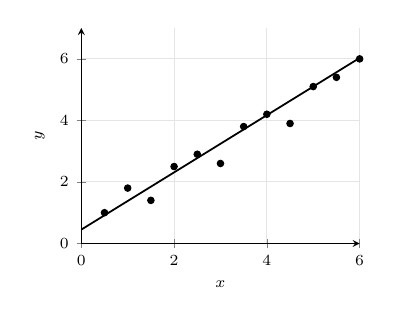
\begin{tikzpicture}[scale=0.8]
        \begin{axis}[
            width=6cm, height=5cm,
            xlabel={$x$}, ylabel={$y$},
            xlabel style={font=\scriptsize},
            ylabel style={font=\scriptsize},
            tick label style={font=\scriptsize},
            xmin=0, xmax=6,
            ymin=0, ymax=7,
            axis lines=left,
            grid=major,
            grid style={gray!20},
        ]
            % Scatter data points
            \addplot[
                only marks,
                mark=*, mark size=1.5pt,
                color=black
            ] coordinates {
                (0.5, 1.0) (1.0, 1.8) (1.5, 1.4)
                (2.0, 2.5) (2.5, 2.9) (3.0, 2.6)
                (3.5, 3.8) (4.0, 4.2) (4.5, 3.9)
                (5.0, 5.1) (5.5, 5.4) (6.0, 6.0)
            };
            % Regression line: y = 0.93x + 0.45
            \addplot[
                thick, color=black,
                domain=0:6, samples=2
            ] {0.93*x + 0.45};
        \end{axis}
    \end{tikzpicture}
\end{center}

One way of doing \emph{linear regression} is via the method of the least squares found in the linear algebra section of this book:

\[
    w = (X^T X)^{-1}X^T y = X^{\dagger}y
\]

But this is computationally very expensive and does not gives us \(b\). An alternative way is by minimizing the \emph{mean squared error} function given by 

\[
    \mathrm{MSE} = J(w,b) = \frac{1}{N} \sum_{i = 1}^{N} (y_i - (wx_i + b))^2
\]

For this we compute the gradient of of \(J(w,b)\)

\[
    J'(w, b) = 
    \begin{bmatrix}
        \frac{\partial J}{\partial w} \\     
        \frac{\partial J}{\partial b} \\     
    \end{bmatrix}
    =
    \begin{bmatrix}
        \frac{1}{N} \sum -2x_i (y_i -(wx_i + b)) \\ 
        \frac{1}{N} \sum -2 (y_i -(wx_i + b))
    \end{bmatrix}
    =
    \begin{bmatrix}
        \frac{1}{N} \sum 2x_i (\hat{y}_i - y_i)) \\ 
        \frac{1}{N} \sum 2 (\hat{y}_i-  y_i)
    \end{bmatrix}
\]

Then by applying gradient descent we can approach a minimum of our function by taking in the direction 
negative to the gradient multiplied by a \emph{learning rate} \(0 < \eta\), giving us the following update step.

\begin{align*}
    w &= w - \eta \frac{\partial J}{\partial w}(w,b) \\     
    b &= b - \eta \frac{\partial J}{\partial b}(w,b)     
\end{align*}

This iterative approach is stopped after a certain number of iterations defined as parameter.

We need to make emphasis that we are having some assumptions such as that the data is \textbf{independent}, there exists a predictable trend, 
the variance of the residuals does not change.

\section{Non-Linear Transformations}

The two algorithms covered until know have the condition that both of them are linear, but 
what if our date can not be linearly separated. We can modify the input variable \(x_i\) 
in a non-linear way to be able to separate the data linearly in another space and then apply our algorithms.

For this purpose, we define the new space \(\mathcal{Z}\) whose elements are \(z_n = \phi(x_n)\), where 
\(\phi: \mathcal{X} \to \mathcal{Z}\) is a non-linear transformation. We also define \(\hat{g}(z) = \text{sign}(\inner{\hat{w}}{z})\).
Finally, our hypothesis set \(\mathcal{H}_{\phi}\) contains functions of the form \(h(x) = \hat{h}(\phi(x))\).

This can become very complex but for 3d or 2d cases with data visualization a non-linear transformation can be found 
using the mathematical technique of looking with your own eyes. 

\section{Logistic Regression}

\emph{Logistic Regression} is a statistical model that in its basic form uses a logistic function to model a binary dependent variable.
This model returns a probability value which can be mapped to two or more discrete classes.

To achieve the desired result we apply a \emph{linear regression} and then apply the \emph{logistic function} to the result to 
squish it between 0 and 1.

The logistic function is defined as

\[
    \theta(s) = \frac{e^s}{1 + e^s} = \frac{1}{1 + e^{-s}}
\]

called the \emph{sigmoid function}, whose domain is \((0, 1)\) and with the properties

\[
    \theta(-s) = 1 - \theta(s), \quad \frac{\partial \theta}{\partial s} = \frac{1}{1 + e^s} \frac{e^{-s}}{1 + e^{-s}}
\]

Note that our original problem with \(\hat{y} = w^Tx + b\) is transformed into 

\[
    h_\theta (x_i) = \frac{1}{1 + e^{- (w^T x_i + b)}}.
\]

Now our function returns the \textbf{probability} of a data point being assigned a corresponding label.

Instead of minimizing the mean squared error, which could be a valid strategy we use the likelihood function which uses 
\(p_i(x_i)^{y_i}(1 - p_i(x_i))^{1 - y_i}\) for penalizing errors more equally.

Let our loss function be 

\[
    L(\theta) = \prod_{n = 1}^N p(x_i)^{y_i}(1 - p(x_i))^{1 - y_i}
\]

where \(p(x_i)\) is the probability of \(x_i\) being assigned the label \(y = 1\) and \(1 - p(x_i)\) the same for \(y = 0\).

We take that expression and modify it using \(h_{\theta}(x_i)\) 

\[
    L(\theta) = \prod_{n = 1}^N (h_\theta(x_i))^{y_i} (1 - h_\theta(x_i))^{1 - y_i}
\]

Taking the logarithm of the likelihood function gives us the log-likelihood:

\[
    \log L(w,b) = - \frac{1}{N} \sum_{i=1}^{N} [y_i \log(h_\theta (x_i)) + (1 - y_i) \log(1 - h_\theta (x_i))]
\]

And this is the function we want to maximize. Note, that this is the \emph{cross entropy loss function}.

\subsection{Gradient of the Cross Entropy Loss Function}

Using the cross entropy we can define our error for logistic regression. By taking the gradient

\[
   \log L(w,b) = - \frac{1}{N} \sum_{i = 1}^{n} [y_i \log(h_\theta (x_i) + (1 - y_i) \log(1 - h_\theta (x_i))]
\]

We get 


\[
    \nabla \log L(\theta) = 
    \begin{bmatrix}
    \frac{\partial \log L(w,b)}{\partial w} \\ 
    \frac{\partial \log L(w,b)}{\partial b}
    \end{bmatrix}
    = 
    \begin{bmatrix}
    \frac{1}{N} \sum_{i=1}^{N} 2x_i\left(\frac{1}{1 + e^{- (w^T x_i + b)}}- y_i\right) \\ 
    \frac{1}{N} \sum_{i=1}^{N} 2\left(\frac{1}{1 + e^{- (w^T x_i + b)}}- y_i\right) 
    \end{bmatrix}
    = 
    \begin{bmatrix}
        \frac{1}{N} \sum_{i=1}^{N} 2x_i(h_\theta(x_i) - y_i)\\ 
        \frac{1}{N} \sum_{i=1}^{N} 2(h_\theta(x_i) - y_i) 
    \end{bmatrix}
\]

In vector form

\[
    \nabla_w \log L(w,b) = \frac{1}{N} X^T (h_\theta(X) - y)
\]

\[
    \nabla_b \log L(w,b) = \frac{1}{N} \sum_{i=1}^{N} (h_\theta(x^i) - y^i)
\]

\subsection{Logistic Regression Algorithm}

\begin{enumerate}

    \item Initialize \(w\) and \(b\) (e.g., to zeros or small random values).

    \item For each iteration until convergence or for a fixed number of iterations:
    
        \begin{enumerate}
        
            \item Compute the predictions for all training examples:
        
                \[
                     y_{\text{pred}} = h_\theta(x^i) = \frac{1}{1 + e^{-(w^T x^i + b)}}
                \]
 
            \item Compute the gradients:

                \[
                    \nabla_w \log L(w,b) = \frac{1}{N} X^T (h_\theta(X) - y)
                \]

                \[
                    \nabla_b \log L(w,b) = \frac{1}{N} \sum_{i=1}^{N} (h_\theta(x^i) - y^i)
                \] 
        
            \item Update the parameters using gradient descent:
        
                \[
                    w \leftarrow w - \alpha \nabla_w \log L(w,b)
                \]
                
                \[
                    b \leftarrow b - \alpha \nabla_b \log L(w,b)
                \]

        \end{enumerate}

    \item After all iterations, output the learned parameters \(w\) and \(b\).

    \item We predict our data by 
    
    \[
        y_{\text{pred}} = h_\theta(X)
    \]

    followed by assigning each prediction a label based on single threshold or a list of ranges.

\end{enumerate}

\section{Decision Trees}

\emph{Decision trees} are used mainly for \emph{regression trees} or classification \emph{decision trees} which 
are used to partition the data into subsets on a purity measurement.

Formally, given a feature vector \(x \in X\) in a \(d\)-dimensional feature space with 
\(R_1, R_2, \dots, R_M\) being disjoint regions \emph{hyper-quadrants} in the feature space. 

The hypothesis \(h(x)\) of a tree is given by the formula 

\[
    h(x) = \sum_{m = 2}^{M} c_m \ind_m (x)
\]

Common purity measurements include: the empirical variance and the Gini impurity.

\subsection{Recursive Binary Splitting}

We previously state an optimization problem, which sadly can not be solved efficiently, instead 
we will approach it with \emph{recursive binary splitting} an algorithm which goes as follows 

\begin{enumerate}

    \item Given \(R_0\) a hyperquadrant with training data \((x_i, y_i)\). Given a feature vector \(x_i = (x_{i1}, \dots, x_{id})\). Also, given 
     \(j \in \{1, \dots, d\}\) as the indexes of the feature and \(s \in \R\) a bias term. 

    \item Define the regions 
    \[
        R_1(j,s) = \{x \mid (x)_j < s, x \in R_0\}
    \]
    \[
        R_2(j,s) = \{x \mid (x)_j \ge s, x \in R_0\}
    \]

    Find \((j, s)\) which minimizes the following 

    \[
        \theta = \min \left(\sum_{i:x_i \in R_1 (j,s)} (y_i - \overline{y_{R_1}})^2 + \sum_{i:x_i \in R_2 (j,s)} (y_i - \overline{y_{R_2}})^2\right) 
    \]

    \item For the next step repeat step one, \(R_0 = R_1\) or \(R_0 = R_2\) depending on the smallest, else terminate.
\end{enumerate}

The termination criteria are for example 

\begin{itemize}
    \item Each leaf which has to be divided has a minimal number of data points contained.

    \item The tree can have maximal depth. 
    
    \item The tree size is limited.
\end{itemize}

\subsection{Regressions Trees}

A \emph{regression tree} divides the feature space into disjoint sub-spaces in such a way that it brings
the value of all labels \(y_i\) for \(x_i \mathcal{D}\) get as as close as possible to the true label \(\overline{y_i} \approx = y_i\). 

The process behind this goal is called \emph{recursive binary splitting} and can be performed in different manners, based on 
how the "purity" of a node is measured. This is of course an optimization in which we want to maximize the purity of our node given a split.

\subsection{Classification Trees}

We can take everything from the regression tree except the cost function. For 
\emph{classification trees} the cost function is given as the label of the specific classes itself.

\textbf{Nomenclature}

\begin{itemize}
    \item \(C\) is the number of classes in the classification problem. 

    \item \(p(i)\) is the probability of the class relative to the complete set.
\end{itemize}

\subsection{Gini Impurity}

Represents the mean probability for a data point being misclassified. \(p(i) = p_i\)

This probability that a data point was misclassified is given by

\[
    \sum_{k \ne i}^{C} p_k = 1 - p_i
\]

The mean is then 

\[
    E_{\text{Gini}}= \sum_{i}^{C}p_i (1 - p_i) = \sum_{i}^{C} p_i - \sum_{i}^{C} p_{i}^2 = 1 - \sum_{1}^{C} p_{i}^{2} 
\]

\subsection{Information Gain in Machine Learning}

Information gain is a measure commonly used in decision tree algorithms such as ID3, C4.5, 
and CART to determine which feature should be used to split the dataset 
at each step. It quantifies how much uncertainty about the class labels is reduced after 
splitting the data based on a particular feature.

\subsection{CART Algorithm}

The \emph{CART} (Classification and Regression Trees) algorithm is a popular decision tree algorithm used for both classification and regression tasks.
The CART algorithm constructs binary trees by recursively splitting the data based on feature values to minimize impurity or variance.

The steps of the CART algorithm are as follows:

\begin{enumerate}

    \item \textbf{Select the Best Split:} For each feature, evaluate all possible split points and calculate the impurity (e.g., Gini impurity for classification or variance for regression) 
    for each split. Choose the feature and split point that results in the lowest impurity.

    \item \textbf{Create Child Nodes:} Split the dataset into two subsets based on the selected feature and split point, creating left and right child nodes.

    \item \textbf{Repeat Recursively:} For each child node, repeat steps 1 and 2 until a stopping criterion is met (e.g., maximum tree depth, minimum number of samples in a node, or no further reduction in impurity).

    \item \textbf{Assign Class Labels or Values:} For classification tasks, assign the most common class label to each leaf node. For regression tasks, assign the mean value of the target variable to each leaf node.
    
\end{enumerate}

\subsection{Variance Reduction}

In regression tasks, the CART algorithm aims to minimize the variance within each node after a split. The variance reduction is calculated as follows: 

\[
    \text{Variance Reduction} = \text{Var}(R) - \left( \frac{N_{left}}{N} \text{Var}(R_{left}) + \frac{N_{right}}{N} \text{Var}(R_{right}) \right)
\]

with 

\[
    \var (Y) = \frac{1}{N - 1} \sum_{i = 1}^{N} (y_i - \overline{y})^2
\]

\subsection{Random Forest}

The \emph{random forest} algorithm is an ensemble learning method that combines multiple decision trees to improve predictive performance and reduce overfitting.

The steps to create a random forest are as follows:

\begin{enumerate}

    \item \textbf{Bootstrap Sampling:} For each tree in the forest, a bootstrap sample is created by randomly sampling the training data with replacement. 
    This means that some data points may be included multiple times, while others may not be included at all.

    \item \textbf{Feature Selection:} At each split in the decision tree, a random subset of features is selected. This randomness helps to decorrelate the trees in 
    the forest, making the ensemble more robust.

    \item \textbf{Tree Construction:} Each decision tree is grown to its maximum depth without pruning. The splitting criteria (e.g., Gini impurity or information gain)
    are used to determine the best splits based on the selected features.

    \item \textbf{Aggregation:} For classification tasks, the final prediction is made by majority voting among all trees in the forest. For regression tasks, the 
    predictions from all trees are averaged to obtain the final output.

\end{enumerate}

\section{Nearest Neighbors Models}

\subsection{Quantifying the Differences between Features}

Examples of metrics:

\begin{itemize}

    \item Euclidean Distance \( d(x ,y) = \metric{x - y}\)

    \item Cosine Similarity \( \mathrm{sim}(x, y) = \frac{x \cdot y}{\metric{x} \metric{y}} \) 

    \item Jaccard Similarity \( \mathrm{sim}(A, B) = \frac{|A \cap B|}{|A \cup B|} \in [0, 1] \)

\end{itemize}

\subsection{Nearest Neighbors}

Given a data-set \(\mathcal{D} = \{(x_1, y_1), \dots, (x_N, y_N)\}\) and a new point \(x\) we want to predict its label \(y\).
We choose a \emph{distance metric} \(d(x, x')\) to quantify the difference between two feature vectors. 

To predict the label of \(x\) we find the \(k\) nearest neighbors of \(x\) in the data-set \(\mathcal{D}\) based on the distance metric \(d\).

Feature vectors in the training set are noted with its distance to \(x\). \(x_{[1]}\) symbolizes the nearest neighbor of 
\(x\), \(x_{[2]}\) the second nearest and so on 

\[
    d(x, x_{[1]}) \le d(x, x_{[2]}) \le \dots d(x, x_{[N]})
\]

The \emph{Nearest Neighbor Model} gives us our final hypothesis is given by :\(g(x) = y_{[1]}(x)\)

\subsection{K-Nearest Neighbors Classification}

The \emph{KNN classification} is a generalization of the \emph{NN model}. 

Given an integer \(k \ge 1\) and \(y \in \{-1, 1\}\) the \emph{k-nearest neighbor} model of binary classification is given by 

\[
    g(x) = \mathrm{sign} \left(\sum_{i = 1}^{k} y_{[i]}(x)\right) 
\]

Note that for \(k = 1\) we get the previous NN model. This is a majority vote model.

\subsection{K-Nearest Neighbor Regression}

The \emph{KNN regression} is determines the label of the feature based on the mean of the 
label of the neighbors

\[
    g(x) = \frac{1}{k} \sum_{i = 1}^{k} y_{[i]}(x)
\]

This is useful when dealing with non binary label sets.

\subsection{KNN Algorithm}

Given a distance metric \(d(x, y)\) we classify our training data using the following steps for each data point \(z\):

\begin{enumerate}

    \item Compute its distance for all other data points \(d(z, v_i)\). 

    \item Sort the distances in ascending order, by also keeping track of the indexes. 

    \item Based on the parameter \(k\) get the distances of the \(k\) closest points. 
    
    \item Depending on the regression or classification apply ont the following formulas 
    
    \[
        \text{Regression:}\, g(x) = \mathrm{sign} \left(\sum_{i = 1}^{k} y_{[i]}(x)\right) \quad \text{Classification:}\, g(x) = \frac{1}{k} \sum_{i = 1}^{k} y_{[i]}(x)
    \]
   
    using the indexes of the \(k\) nearest neighbors for the getting the corresponding labels.

\end{enumerate}

\section{Support Vector Machines}

\emph{Support vector machines} are a family of algorithm which use the perceptron as a basis for classifying points into classes using a hyperplane 

\[
    w_0 + w_1 x_1 + \dots + w_p x_p = 0
\]

But this time we also define a region defined by the normal vectors of the hyperplane and define it as our \emph{margin}, which we will try to optimize 
to be as large as possible.

As starting point we take the perceptron we already defined with \(b = w_0\) being the bias term

\[
    y_k = \mathrm{sign}(w^T x + b) = \mathrm{sign}(\tilde{w}^T\tilde{x}), \,  y_k \in \{-1, 1\}
\]

\subsubsection{Rescaling of the Signal}

The term inside our \emph{sign} function, the signal, can be rescaled without changing the 
result of the classification. Due to the property of the sign function \(\mathrm{sign}(\alpha s) = \mathrm{sign}(s)\) 
for any \(\alpha > 0\). 

\[
    y_k = \text{sign}(w^T x_k + b) \implies y_k (w^T x_k + b) > 0
\]

The behavior of the rescaling acts differently on if the data point is in the margin or not. 

\[
    y_k(w^T x_k + b) = 1 \quad \text{ for points in the margin}
\]

\[
    y_k(w^T x_k + b) > 1 \quad \text{ for points outside the margin}
\]

\subsubsection{Width of the Margin}

Given two points \(x_1, x_2\) lying on the margin with different labels. Therefore,

\begin{align*}
    (I)  w^T x_1 + b &= 1 \\ 
    (II) w^T x_2 + b &= -1
\end{align*}

Then we get 

\[
    w^T (x_1 - x_2) = 2
\]

The \emph{width} of the margin \(r\) is given by the projection of the vector \(x_1 - x_2\) onto the
normal vector \(\frac{w}{\|w\|}\)

\[
    r = \frac{w^T (x_1 - x_2)}{\|w\|} = \frac{2}{\|w\|}
\]

Therefore, to maximize the width of the margin we have to minimize \(\frac{1}{2}\|w\|\).

\subsection{Hard Margin SVM}

A \emph{hard margin SVM:} is a perceptron with maximal margin and no misclassifications.

Like previously stated, to maximize the width \(r = \frac{2}{\|w\|}\) of the margin we have to minimize \(\frac{1}{2}\|w\|\).

Formally, we want to solve the following optimization problem 

\emph{Minimize:} \(\frac{1}{2}\|w\|^2\) under \(N\) \emph{constraints} 

\emph{Maximize:} \(y_n (w^T x_n + b) \ge 1, (n = 1, \dots, N)\)

We will skip the derivation of the final solution, which is done via \emph{Karush-Kuhn-Tucker conditions}. Now, 
we have a \emph{dual optimization problem} 

\[
    \max \left(- \frac{1}{2} \sum_{n = 1}^{N}\sum_{m = 1}^{N} y_n y_m \alpha_n \alpha_m x_n^T x_m + \sum_{n = 1}^{N} \alpha_n \right)
\]

under the condition 

\[
    \sum_{n = 1}^{N} \alpha_n y_n = 0
\]

In the primary problem we had 

\[
    y_n = \text{sign}(w^T x_n + b)
\]

Now in the dual problem we have

\[
    y_i = \text{sign} \left(\sum_{n = 1}^{N} \alpha_n y_n x_n^T x_i + b \right)
\]

with \(\alpha\) being our solution vector with dimension \(N\).

Some components of \(\alpha\) will be zero, and the others positive, due to it being \emph{sparse}. Therefore 

\[
    y_i = \text{sign} \left(\sum_{k \in \mathcal{s}} \alpha_k y_k x_k^T x_i + b \right)
\]

with \(\mathcal{S} = \{j \mid \alpha_j \ne 0, j = 1, \dots, N\}\).

Finally, the data points \(x_k\) with \(\alpha_k \ne 0\) are called \emph{support vectors} 
and the \(a_k \ne 0 \) the \emph{support values}.

\subsection{Soft Margin Support Vector Machine}

The idea of \emph{soft margin SVM} is to allow misclassifications but penalize them in the optimization problem.
To get the best soft margin we can use cross validation.

Formally, we want to solve the following optimization problem: 

\emph{Minimize:} \(\frac{1}{2} w^T w + C \sum_n \xi_n\) under \(N\) \emph{constraints} 

In other words, maximize \(\frac{1}{2}w^Tw\), the width of the margin, minimize \(\sum_n \xi_n\), the total error.

With the constraint \(y_n (w^T x_n + b) \ge 1 - \xi_n, (n = 1, \dots, N)\)

\[
    \xi_n = \max (0, 1 - y_n (w^T x_n + b))
\]

Thus, 

\[
    \frac{1}{2} w^T w + C \sum_n \max (0, 1 - y_n (w^T x_n + b))
\]

with \(C\) is our regularization parameter.

Our \emph{dual optimization problem} is given by

\[
    \max \left(- \frac{1}{2} \sum_{n = 1}^{N}\sum_{m = 1}^{N} y_n y_m \alpha_n \alpha_m x_n^T x_m + \sum_{n = 1}^{N} \alpha_n \right)
\]

under the conditions

\[
    \sum_{n = 1}^{N} \alpha_n y_n = 0, 0 \le \alpha_n \le C \forall n
\]

Also, 

\[
    y_i = \text{sign} \left(\sum_{n = 1}^{N} \alpha_n y_n x_n^T x_i + b \right)
\]

\subsection{Non-Linear Support Vector Machines}

We will allow non-linear feature Transformations \(x \to \Phi(x)\) 

\[
    x_n^Tx_i \to \Phi(x_n)^T \Phi(x_i)
\]

Now our \(y_i\) becomes 

\[
    y_i = \text{sign} \left(\sum_{n = 1}^{N} \alpha_n y_n \Phi(x_n)^T \Phi(x_i) + b \right)
\]

Let us also \(K:= \Phi(x_n)^T \Phi(x_i)\)

\subsubsection{Kernel Trick}

The \emph{kernel trick} allows us to compute the inner product in the transformed feature space without explicitly performing the transformation.
For that we use so-called \emph{kernel functions, K} to use as inner products in the feature space. We are basically using 
mathematical elegance to use high dimensional spaces without paying the computational cost.

The kernel functions must satisfy the following properties \emph{Mercer's Theorem}:

\(K\) is a \emph{kernel} if the kernel matrix \(K\) is symmetric and positive semi-definite for any set of input data points. 

\[
    x^T K x \ge 0 \quad K = K^T
\]

\textbf{Common Kernel Functions:}

\begin{itemize}

    \item \emph{Linear:} \(k(x,y) = x^T y\)
    
    \item \emph{Polynomial:} \(k(x,y) = (x^T y + c)\)

    \item \emph{RBF:} \(k(x,y) = \exp( -\gamma \|x -  y \|^2)\)
    
    \item \emph{Sigmoid:} \(k(x,y) = \tanh( \gamma x^Ty + c)\)

\end{itemize}

We can also give parameters \(\alpha, \beta\) for \(k(\beta + \alpha x^T, y)\)

\textbf{Example:}

Given \(\Phi(x_1, x_2) = (1, \sqrt{2}x_1, \sqrt{2}x_2, x_1^2, \sqrt{2}x_1x_2, x_2^2)\) we 
get for 

\[
    \langle \Phi(x), \Phi(y)\rangle = 1^2 +  \sqrt{2}x_1\sqrt{2}y_1 + \sqrt{2}x_2\sqrt{2}x_2 + x_1^2 y_1^2 + \sqrt{2}x_1x_2 \sqrt{2}y_1y_2 + x_2^2 y_2^2
\]

The following kernel by simplifying

\[
    \langle \Phi(x), \Phi(y)\rangle = 1 + 2x^T y + (x^Ty)^2 = (1 + x^Ty)^2 = k(x,y)
\]

Generalized \((d + x^Ty)^2 \)

\subsection{The Radial Kernel}

The \emph{radial basis function (RBF) kernel} is defined as 

\[
    K(x, y) = \exp\left(- \frac{\|x - y\|^2}{2\sigma^2}\right)
\]

where \(\sigma > 0\) is a parameter that controls the width of the Gaussian function, and 
\(\sigma\) is the standard deviation of the Gaussian distribution.

The infinite-dimensional property comes from the fact that the RBF kernel can be expressed as an infinite series expansion,

\[
    K(x, y) = \sum_{n=0}^{\infty} \frac{1}{n!} \left(-\frac{\|x - y\|^2}{2\sigma^2}\right)^n
\]

\subsection{Least Squares Support Vector Machine}

This is a simplified version of the soft margin SVN. 

Formally, 

\emph{Primary Optimization Problem:}

\emph{Minimize:} \(\frac{1}{2} w^T w + \frac{\gamma}{2} \sum_n^N e_n^2\) under \(N\) constraints.

\[
    y_n(w^t x_n + b) = 1 - e_n, 
\]

with 

\[
    e_n^2 = y_n^2 (y_n - (w^T x_n + b))2 = (y_n - (w^T x_n + b))
\]

The Lagrangian we get is 

\[
    \mathcal{L} = \frac{1}{2} w^T w + \frac{\gamma}{2} \sum_n^N e_n^2 - \sum_{n = 1}^{N} \alpha_n [y_n (w^T x_n + b) - 1 + e_n]
\]

Apply \(\nabla_{w, b, e, \alpha} \mathcal{L} = 0\)

\begin{align*}
    \textbf{I } \frac{\partial \mathcal{L}}{\partial w} &= w - \sum_{k = 1}^{N} \alpha_k y_k x_k = 0 \iff w = \sum_{k = 1}^{N} \alpha_k y_k x_k \\ 
    \textbf{II } \frac{\partial \mathcal{L}}{\partial b} &= - \sum_{k = 1}^{N} \alpha_k y_k = 0 \iff  y^t \vec{\alpha} = 0 \\ 
    \textbf{III } \frac{\partial \mathcal{L}}{\partial e} &= \gamma e_k - a_k  =0 \iff \alpha_k = \gamma e_K  \iff e = \frac{1}{\gamma} \vec{\alpha}\\ 
    \textbf{IV } \frac{\partial \mathcal{L}}{\partial \alpha_k} &= - y_k (w^T x_k + b) + 1 - e_k \iff y_k (w^T x_k + b) + e_k = 1 \forall k
\end{align*}

Now let us combine our results 

\begin{align*}
    \textbf{I } w = \sum_{k = 1}^{N} \alpha_k y_k x_k \\ 
    \textbf{II }  y^t \vec{\alpha} = 0 \\ 
    \textbf{III }  e = \frac{1}{\gamma} \vec{\alpha}\\ 
    \textbf{IV }  y_k (w^T x_k + b) + e_k = 1 \forall k
\end{align*}

Substitute I and III in IV 

\begin{align*}
    &y_k (w^T x_k + b) + e_k = 1 \forall k \\ 
    &\iff y_k (\sum_{j = 1}^{N} \alpha_j y_j x_j^T x_k + b) +  \frac{1}{\gamma} \alpha_k = 1 \forall k \\ 
    &\iff y_k b + \sum_{j = 1}^{N} \alpha_j y_j x_j^T x_k y_k +  \frac{1}{\gamma} \alpha_k = 1 \forall k 
\end{align*}

Now replace the dot product with the kernel function 

\[
    \iff \text{V } yb + (yyT \cdot K) \vec{a} + \frac{1}{\gamma} I\vec{a} = 1
\]

The only results left to use are II and V which we can combine into 

\[
    A = 
    \begin{bmatrix}
        0 & y^T \\ 
        y & \Omega + \frac{1}{\gamma} I
    \end{bmatrix} 
\]

After this process we get 

\[
    y_i = \mathrm{sign}(w^T x_i + b) \implies \mathrm{sign}\left(\sum_{k = 1}^{N} \alpha_k y_k x_k^T x_i + b\right)
\]

We can apply our kernel function and get

\[
    y_i = \mathrm{sign}\left(\sum_{k = 1}^{N} \alpha_k y_k K(x_k, x_i) + b\right)
\]


\subsubsection{Least Square Support Vector Machine Implementation}

\begin{enumerate}

    \item Implement the kernel function, typically 
    \[
        K(x_k, x_i) = \exp\left(- \frac{\|x_k - x_i\|^2}{2\sigma^2}\right)
    \]

    \item Compute the \(n \times n\) matrix \(\Omega = yy^T \cdot K\) with \(y\) being the label vector and \(K\) the  
    kernel matrix.

    \item Find the matrix   
    \[
        A = 
        \begin{bmatrix}
            0 & y^T \\ 
            y & \Omega + \frac{1}{\gamma} I
        \end{bmatrix} 
    \]

    \item Invert \(A\) and get \(b\) and \(\vec{\alpha}\)     
    \[
        \begin{bmatrix}
            b \\ 
            \vec{\alpha}
        \end{bmatrix}
        = 
        A^{-1} 
        \begin{bmatrix}  0  \\ 1 \end{bmatrix}
    \]

    \item Predict the labels 
    \[
        y_i = \mathrm{sign}\left(\sum_{k = 1}^{N} \alpha_k y_k K(x_k, x_i) + b\right)
    \]

   

\end{enumerate}

\section{Dimension Reduction}

The \emph{curse of dimensionality} is a concept that describes the problems which arise when dealing with hight-dimensional data. A high 
number of features (dimensions) leads to an increase in the complexity of the model as well as the computational cost. Also, in data science it 
is important to be able to visualize the data, which is not possible in high dimensions. Therefore, we want to reduce the number of features while 
preserving as much information as possible.

\subsection{Average Vector}

Given \(N\) features vectors with \(D\) features. The \emph{average vector} is given 
by

\[
    \overline{x} = \frac{1}{N} \sum_{n = 1}^{N} x_n
\]

This vector is used to center the data by subtracting it from each feature vector. This vector has as its components the mean of the corresponding feature across all feature vectors.

\subsubsection{Z Scoring}

Given \(\overline{X}\) as the mean and \(\sigma\) as the standard deviation of \(X\). The standardize feature 
\(Z\) (z-score) is given by 

\[
    Z = \frac{X - \overline{X}}{\sigma}
\]

In practice, data are often organized in matrices where each column represents a feature.
In this case, standardize each feature by transforming every column separately so that it has mean 0 and variance 1 (i.e., standard deviation 1).


\subsection{Dimension Reduction Principal Component Analysis PCA}

\emph{PCA (Principal Component Analysis)} finds new axes called components for the data, such that the data show the largest possible variance along these axes.
In other words, PCA looks for directions in which the data vary the most.

Axes along which the data have little, or almost no variance can usually be ignored, because they contain little useful information. 

When projecting our points onto a new axis we use the projection formula 

\[    
	a' = \mathrm{Proj}_{b}(a) = \inner{a}{b}b.
\]

We can use the the term \(\inner{a}{b}\) as the measure of information preserved between the two vectors \(a\) and \(a'\). This is 
maximal when they are orthogonal and maximal when they are parallel. 

Hence, we want to maximize the sum of the inner products between the original data and the projected data onto the directions \(u\) which 
while minimizing the the loss of information.

\[
    \max \sum_i \inner{x_i}{u}^2 = \max \sum_i (x_i^T u)^2
\]

Note that we still do not know in which direction \(u\) we want to project our data. For this we can manipulate the previous expression 

\begin{align*}
    \max \sum_i (x_i^T u)^2 &= \max \sum_i (x_i^T u)(x_i^T u) \\ 
    &= \max \sum_i u^T x_i x_i^T u \\
    &= \max u^T \left( \sum_i x_i x_i^T \right) u 
\end{align*}

Note the covariance matrix inside

\[
    S = \frac{1}{N} \sum_i (x_i - \overline{x})(x_i - \overline{x})^T 
\]

If we assume that the data is centered around the mean, then we can write

\[
    S = \frac{1}{N} \sum_i x_i x_i^T = X^TX
\]

For

\[
    X =
    \begin{bmatrix}
       - & X_1 & -\\ 
       - & X_2 & - \\ 
        & \vdots & \\ 
      -  & X_n & - 
    \end{bmatrix}
\]

In our optimization problem we can replace the covariance matrix and get

\[
    \max (u^T S u)
\]

With the constraint 

\[
    u_i^T u_i = 1 \iff 1 - u_i^T u_i = 0  
\]


We also have the constraint that \(u\) is a unit vector, so we can write the optimization problem as

\[
    \max (u^T S u) \quad \text{subject to } u^T u = 1
\]

Now using the method of Lagrange multipliers we can write the Lagrangian as

\[
    \mathcal{L}(u, \lambda) = u^T S u - \lambda (u^T u - 1)
\]

Taking the gradient and setting it to zero gives us

\[
    \nabla_u \mathcal{L} = 2Su - 2\lambda u = 0 \implies Su = \lambda u
\]

Which is an eigenvalue problem. The solution \(u\) is an eigenvector of the covariance matrix \(S\) and \(\lambda\) is the corresponding eigenvalue.

Because we want to maximize \(u^T S u\), we need to choose the eigenvector corresponding to the largest eigenvalue. 
This eigenvector is called the \emph{first principal component}.

From 

\begin{align*}
    S u_i &= \lambda_i u_i \\ 
    u_i^T S u_i = \lambda_i
\end{align*}

Depending on how many dimensions we want to reduce to, we can choose the eigenvectors corresponding to the largest eigenvalues.

\subsubsection*{Projection}

Each of our principal components represents a direction in our high dimensional space. Given our data set \(X \in \R^{n \times p}\) 
and our matrix of \(k\) principal components \(W^T \in \R^{k\times p}\); the projection of our data onto the components is given by 

\[
    Z = XW^T ,\quad Z \in \R^{n \times k}
\]

This comes from the fact that given our projection:

\[
    \mathrm{Proj}_{u_i}(x) = u_i^T x u_i \iff u_i^T u_i = 1.
\]

When we multiply our matrices \(X\) and \(W\)

\[
    \begin{bmatrix}
        - & X_1 & -\\ 
        - & X_2 & - \\ 
        & \vdots & \\ 
        -  & X_n & -
    \end{bmatrix}
    \begin{bmatrix}
        - & u_1 & -\\ 
        - & u_2 & - \\ 
        & \vdots & \\ 
        -  & u_k & -
    \end{bmatrix}^T
    = 
    \begin{bmatrix}
        \inner{X_1}{u_1} & \inner{X_1}{u_2} & \dots & \inner{X_1}{u_k} \\
        \vdots & \vdots & \ddots & \vdots \\
        \inner{X_n}{u_1} & \inner{X_n}{u_2} & \dots & \inner{X_n}{u_k}
    \end{bmatrix}
\]

Which essentially describes the our vector as a liner combination:

\[
    Z_1 = \inner{X_1}{u_1} u_1 +  \inner{X_1}{u_2} u_2 + \dots + \inner{X_1}{u_k} u_k = \sum_{i = 1}^{k} \inner{X_1}{u_i} u_i 
\]

Note that we are using the row vectors of \(X\) and the transpose of the matrix of principal components \(W^T\) to get the projection, because of 
the way most software libraries implement matrices as arrays of row vectors.

\subsubsection*{Variance Derivation}

Alternatively to our previous derivation of the PCA, we can accomplish the same result by:

First taking our projection

\[
    \mathrm{Proj}_{u_i}(x_j) = u_i^T x_j u_i
\]

Then taking the mean vector projected \(u_{i}^T \overline{x} u_i\) and then using the variance formula for 
the variance of the projections with our unit vector \(u_i\):

\begin{align*} 
    \frac{1}{N} \sum_{i = 1}^{N} (u_i^T x_j -  u_i^T \overline{x})^2 &= \frac{1}{N} \sum_{i = 1}^{N} [u_i^T (x_j - \overline{x})]^2 \\ 
    &= \frac{1}{N} \sum_{i = 1}^{N} u_i^T (x_j - \overline{x}) u_i^T(x_j - \overline{x}) \\ 
    &= \frac{1}{N} \sum_{i = 1}^{N} u_i^T (x_j - \overline{x}) (u_i^T(x_j - \overline{x}))^T \\ 
    &= \frac{1}{N} \sum_{i = 1}^{N} u_i^T (x_j - \overline{x}) (x_j - \overline{x})^Tu_i \\ 
    &=  u_i^T S u_i 
\end{align*}

The rest of the derivation is the same as by the previous.

\subsection{Explained Variance}

If we divide each eigenvalue by the sum of all eigenvalues we get the \emph{explained variance EV} of each principal component.

\[
    \mathrm{PVE} = \frac{\lambda_k}{\sum_{j = 1}^{D} \lambda_j}
\]

This tells us how much of the variance in the data is explained by each principal component. We can use this to decide how many principal components to 
keep based on a desired level of explained variance.

\subsection{Covariance Optimization}

For the computation of our principal components, we have been using the expression \(S = X^Tx\). Although, this 
is mathematically correct, for certain data sets with more features than samples this can become a really big matrix. To improve 
this problem we make use of the one of the following properties of our eigenvalue problem.

\begin{align*}
    S u _i &= \lambda_i u_i \\
    X^T X u_i &= \lambda_i u_i \\ 
    X X^T X v_i &= X \lambda_i X u_i \\ 
    (X X^T)(X u_i) &=  \lambda_i (X u_i) \\ 
    (X X^T)v_i &=  \lambda_i v_i
\end{align*}

This means that our eigenvalue and eigenvectors are the same if we instead of the \emph{feature covariance matrix} we use the \emph{sample covariance matrix} \(XX^T\).

\subsubsection*{Big Picture For the Algorithm}

We want to reduce the number of features from \(D\) to \(M < D\) or just inspect our data for the features which contribute the most 
variance.

The algorithm goes as following: 

\begin{enumerate}

    \item We have \(N\) feature vectors with \(D\) features each.  

    \item Compute the average vector  \(\overline{x} = \frac{1}{N} \sum_{n = 1}^{N} x_n\)
    
    \item Subtract the mean \(B = X - \overline{X}\)
   
    \item We have a \(D \times D\) covariance matrix \(S = B^T B\) or \(BB^T\) depending on the number of samples and features.

    \item We compute the eigenvalues and eigenvectors of \(S\)

    \item We sort the eigenvalues with their corresponding eigenvectors in decreasing order and take the first \(M\) eigenvectors 

    \item These eigenvectors form the new basis for the feature space. With which we can project our feature vectors.

\end{enumerate}

\subsection{Kernel PCA}

This is an extension of PCA to non-linear feature spaces via the kernel trick.

\subsubsection{Reformulation of the PCA with Non-Linear Features}

The covariance matrix \(S = \frac{1}{N} \sum_{n = 1}^{N} (x_n - \overline{x})(x_n - \overline{x})^T\) can 
be reformulated with \(x_i \to \Phi(x_i)\) to 

\[
    S = \frac{1}{N} \sum_{n = 1}^{N} (\Phi(x_n) - \overline{\Phi(x)})(\Phi(x_n) - \overline{\Phi(x)})^T
\]

Assume that the features vectors are centered in the feature space, i.e. \(\overline{\Phi(x)} = 0\). 
Then we have

\[
    S = \frac{1}{N} \sum_{n = 1}^{N} \Phi(x_n) \Phi(x_n)^T
\]

\subsubsection{Eigenvector as Linear Combination of the transformed Features}

\begin{align*}
    S u_j &= \lambda_j u_j  \\ 
    S u_j &= \frac{1}{N} \sum_{n = 1}^{N} \Phi(x_n) \Phi(x_n)^T u_j  \\ 
    &= \frac{1}{\lambda_j N} \sum_{n = 1}^{N} \Phi(x_n) (\Phi(x_n)^T u_j)  \\
    &= \frac{1}{\lambda_j N} \sum_{n = 1}^{N} \Phi(x_n)^T u_j (\Phi(x_n))  \\
    &= \sum_{n = 1}^{N} \left( \frac{1}{\lambda_j N} \Phi(x_n)^T u_j \right) \Phi(x_n) \\ 
    &= \sum_{n = 1}^{N} a_{ji} \Phi(x_i)
\end{align*}

with \(u_j = \sum_{l} \alpha_{jl} \Phi(x_l)\)

Because we can express the eigenvectors as a linear combination of the transformed features, we can 
find the coefficients \(\alpha_{jl}\) instead of \(u_j\). 

\subsubsection{Find the Eigenvectors}

\begin{align*}
    \frac{1}{N} \sum_{i} \Phi(x_i) \Phi(x_i)^T \sum_{l} \alpha_{jl} \Phi(x_l) &= \lambda_j \sum_{l} \alpha_{jl} \Phi(x_l) \\
    \frac{1}{N} \sum_{i} \Phi(x_i) \left( \sum_{l} \alpha_{jl} \Phi(x_i)^T \Phi(x_l) \right) &= \lambda_j \sum_{l} \alpha_{jl} \Phi(x_l) \\
    \frac{1}{N} \sum_{i} \Phi(x_i) \left( \sum_{l} \alpha_{jl} K(x_i, x_l) \right) &= \lambda_j \sum_{l} \alpha_{jl} K(x_k, x_l) \\
    \frac{1}{N} KK \vec{\alpha}_j &= \lambda_j K \vec{\alpha}_j \\
     K \vec{\alpha}_j &= N \lambda_j K \vec{\alpha}_j
\end{align*}

Therefore, we have to solve the following eigenvalue problem

\[
    K \vec{\alpha}_j = N \lambda_j \vec{\alpha}_j
\]

Which we reformulate to 

\[
    K \vec{\alpha}_j = \hat{\lambda_j}\vec{\alpha}_j
\]

The coefficients \(\alpha_j\) are the components of the eigenvectors of the kernel matrix \(K\). 

\subsubsection{Normalization of the Eigenvectors}

To normalize the eigenvectors \(u_j\) we have to impose the condition 

\[
    u_j = \sum_{l} \alpha_{jl} \Phi(x_l) \implies \hat{u} = \sum_{l} \hat{\alpha_{jl}} \Phi(x_l) = \hat{u_j^T} u_j^T = 1 \forall j
\]

This gives us

\[
    \sum_k \sum_l \hat{\alpha_{jk}} \hat{\alpha_{jl}} K(x_k, x_l) = 1 \forall j
\]

Which can be reformulated to

\[
    \hat{\vec{\alpha}_j^T} \hat{\lambda_j} \hat{\vec{\alpha}}_j = 1 \forall j \implies \|\hat{\vec{\alpha}}_j\| = \frac{1}{\sqrt{\hat{\lambda_j}}}
\]

With 

\[
    \vec{\alpha_j} \to \hat{\vec{\alpha}}_j = \frac{\vec{\alpha_j}}{\sqrt{\hat{\lambda_j}}} \frac{\vec{\alpha}_j}{\|\vec{\alpha}_j\|}
\]

\subsubsection{Projection onto the KPCA Axis}

\begin{align*}
    \Phi(x)^T u_j &= \Phi(x)^T \sum_{l} \alpha_{jl} \Phi(x_l) \\
    &= \sum_{l} \alpha_{jl} \Phi(x)^T \Phi(x_l) \\
    &= \sum_{l} \alpha_{jl} K(x, x_l)
\end{align*}

\subsubsection{Centering of the Features}

We assumed that the features where centered in the transformed feature space. Now we want to normalize them.

Given 

\[
    \hat{\Phi}(x_i) = \Phi(x_i) - \frac{1}{N} \sum_{l} Phi(x_l)
\]

and the kernel function

\begin{align*} 
    K(x_i, x_j) &= \hat{\Phi(x_i)^T} \hat{\Phi(x_j)} \\ 
    &= \left( \Phi(x_i) - \frac{1}{N} \sum_{l} \Phi(x_l) \right)^T \left( \Phi(x_j) - \frac{1}{N} \sum_{l} \Phi(x_l) \right) \\
    &= K(x_i, x_j) - \frac{1}{N} \sum_{l} K(x_i, x_l) - \frac{1}{N} \sum_{k} K(x_k, x_j) + \frac{1}{N^2} \sum_{k,l} K(x_k, x_l)
\end{align*}

Simplified 

\[
    \hat{K} = K - 1_N K - K 1_N + 1_N K 1_N
\]

where \(1_N\) is the \(N \times N\) matrix with all entries equal to \(\frac{1}{N}\). 

\subsubsection{Kernel PCA Algorithm}

Now we can summarize the K-PCA algorithm

\begin{enumerate}

    \item Choose a kernel function \(K(x, y)\) and compute the kernel matrix \(K\) with entries \(K_{ij} = K(x_i, x_j)\).

    \item Center the kernel matrix to obtain \(\hat{K}\) using \(\hat{K} = K - 1_N K - K 1_N + 1_N K 1_N\)

    \item Solve the eigenvalue problem \(\hat{K} \vec{\alpha}_j = \hat{\lambda}_j \vec{\alpha}_j\) to find the eigenvalues \(\hat{\lambda}_j\) and eigenvectors \(\vec{\alpha}_j\).

    \item Normalize the eigenvectors \(\vec{\alpha}_j \to \frac{1}{\sqrt{\hat{\lambda}_j}} \frac{\vec{\alpha}_j}{\|\vec{\alpha}_j\|}\)

    \item Project the data points onto the K-PCA axes using
    \[
        \Phi(x)^T \hat{u_j} = \sum_{l} \hat{\alpha_{jl}} K(x, x_l)
    \]

\end{enumerate}

\subsection{Multidimensional Scaling MDS}

\emph{Multidimensional Scaling (MDS)} is a family of procedures for the visualization an dimension reduction of features.

Given the pairwise distances of \(N\) vectors in matrix form 

\[
    D = (d_{i,j})_{i,j}^n = \delta_{i,j}
\]

In this classical approach \(d_{i,j}\) represent the distances in the low-dimensional configuration, \(\delta_{i,j}\) the observed distances or dissimilarities and 
\(\hat{d}_{i,j}= f(\delta_{i,j})\) the disparities from our data \(X\), which we do not know and want to find \(X\).

We take our matrix \(D\) and square its entries giving us our \emph{Gram matrix}:

\[
    \tilde{D} = (d_{i,j}^2)_{i,j}^n
\]

Then, we construct our matrix \(B\) for which the following holds:

\[
    B = X X^T, \quad b_{i, j} = \inner{x_i}{x_J}
\]

Using the fact tha twe can write our inner products as 

\[
    \inner{x_i}{x_j} = \frac{1}{2} (\inner{x_i}{x_i} + \inner{x_j}{x_j} - d_{i, j}^2)
\]

we writ \(B\) as

\[
    B = - \frac{1}{2} H \tilde{D} H, \quad H = I - \frac{1}{N} \vec{1} \vec{1}^T
\]

and \(H\) is our \emph{double centering matrix} which subtracts both the row and column mean.

Finally reconstruct \(X\) from using te eigendecomposition with \(V\) as the matrix of eigenvectors and \(\Lambda\) the eigenvalue matrix:

\[
    B = V \Lambda V^t
\]

We get 

\[
    X = V \sqrt{B} = 
    \begin{bmatrix}
        \sqrt{\lambda_1} v_1 & \dots & \sqrt{\lambda_k} v_1
    \end{bmatrix}
\]

Depending on the number of dimensions we want to keep, we can use a certain number of sorted eigenvalues with their corresponding 
eigenvectors to control the dimension reduction,

The idea is similar to PCA, but instead of using correlation between samples, we use the distance/metric to group of samples. Choosing the right 
metric for the method is part of the art. As an important note, the previously discussed method only works with the euclidean distance; for a generalization with any metric 
there is an alternative algorithm.

\subsection{Explained Distance Matrix}



\subsubsection{Euclidean Constraint}

The reason that our distance matrix has to be build using the Euclidean metric is due to the loss of positive definiteness. If \(B = XX^T\) then 

\[
    a^T B a = a^T XX^T a = (Xa)^T(Xa) \ge 0, \ \forall a
\]

Which guarantees positive eigenvalues. Negative eigenvalues lead to non real matrices when reconstructing our data.

This is mostly not a problem in the praxis, due to the negative eigenvalues and they associated eigenvectors are discarded during the algorithm, but 
this can limits the possibilities of projecting our data; meaning more lose of information.

\subsection{Linear Discriminant Analysis}

The goal of the \emph{linear discriminant analysis} is to find directions \(u_1, u_2, \ldots, u_k\) in the classes such they can be best separated. 

For the direction \(u_1\) with the projection of some data point \(x_i\) onto that direction defined as

\[
    \hat{x_i} = u_1^T x_i
\]

Let 

\[
    m^{(k)} = \frac{1}{N_k} \sum_{n \in \mathcal{C}_k} x_n
\]

be the \emph{mean vector} of class \(k\). 

The projection onto \(u_1\) is given by 

\[
    \hat{m}^{(k)} = u_1^T m^{(k)}
\]

\subsubsection*{Within-Class Scatter}

For quantifying the separation of the points projected onto \(u_1\) we define the following
the \emph{within-class scatter} as 

\begin{align*}
    s_w^2 &:= \sum_{n \in \mathcal{C}_k} (\hat{x}_n - \hat{m}^{(k)})^2\\ 
    &= \sum_{n \in \mathcal{C}_k} (u_1^T x_n - u_1^T m^{(k)})^2 \\
    &= u_1^T \left[ \sum_{n \in \mathcal{C}_k} (x_n - m^{(k)})(x_n - m^{(k)})^T \right] u_1 \\ 
    &= u_1^T S_{wk} u_1  
\end{align*}

The \emph{total scatter} for two classes is given by

\begin{align*}
    s_1^2 + s_2^2 &= u_1^T (S_{w1} + S_{w2}) u_1 \\
    &= u_1^T S_W u_1
\end{align*}

For \(n-\)classes we have 

\[
    S_W = \sum_{k = 1}^{n} S_{wk} = \sum_{k = 1}^{n} \sum_{n \in \mathcal{C}_k} (x_n - m^{(k)})(x_n - m^{(k)})^T
\]

\subsubsection*{Between-Classes Scatter}

The quantification of the separation between the middle points, called the 
\emph{between-classes-scatter} is given by 

\begin{align*}
    (\hat{m}^{(1)} - \hat{m}^{(2)})^2 &= (u_1^T m^{(1)} - u_1^T m^{(2)})^2 \\
    &= u_1^T (m^{(1)} - m^{(2)})(m^{(1)} - m^{(2)})^T u_1 \\
    &= u_1^T S_b u_1
\end{align*}

\[
    S_b = (m^{(1)} - m^{(2)})(m^{(1)} - m^{(2)})^T
\]

where \(m^{(1)}\) and \(m^{(2)}\) are the mean vectors of class 1 and class 2. 

\subsubsection{Fisher Discriminant}

The \emph{Fisher Discriminant} is the ratio of the between-class scatter and the within-class scatter.

\[
    J(u_1) = \frac{u_1^T S_b u_1}{u_1^T S_W u_1} = \frac{(u_1^T (m^{(1)} - m^{(2)})(m^{(1)} - m^{(2)})^T u_1)}{u_1^T S_W u_1}
\]

We want to maximize \(J(u_1)\). This means to find the direction \(u_1\) such that the between-class scatter is maximized and the 
within-class scatter is minimized. To accomplish this we take the gradient and set it to zero. 

\begin{align*} 
    \frac{d J(u_1)}{du_1} &= u_1^T S_W u_1 \frac{d}{du_1} (u_1^T S_b u_1) - u_1^T S_b u_1 \frac{d}{du_1} (u_1^T S_W u_1) \\ 
    &= 2 S_b u_1 (u_1^T S_W u_1) - 2 S_W u_1 (u_1^T S_b u_1) = 0 \quad \text{ divide by } 2 (u_1^T S_W u_1)\\
    &\iff S_b u_1 = \frac{u_1^T S_b u_1}{u_1^T S_W u_1} S_W u_1 \\
    &\iff S_b u_1 = J(u_1) S_W u_1 \\ 
    &\iff (S_W^{-1} S_b) u_1 = J(u_1) u_1
\end{align*}

We arrive at an eigenvalue problem where \(u_1\) is the eigenvector of \(S_W^{-1} S_b\) with the corresponding 
eigenvalue \(J(u_1)\).

\subsubsection{Linear Discriminant Algorithm}

\begin{enumerate}

    \item Compute the within-class scatter matrix \(S_W\) and the between-class scatter matrix \(S_b\).

    \item Solve the eigenvalue problem \((S_W^{-1} S_b) u = \lambda u\) to find the eigenvalues \(\lambda\) and eigenvectors \(u\).

    \item Sort the eigenvectors by their corresponding eigenvalues in descending order.

    \item Select the top \(k\) eigenvectors to form a projection matrix \(W\).

    \item Project the original data points onto the new subspace using \(z_i = W^T x_i\).   

\end{enumerate}

\section{Naive Bayes}

The \emph{naive Bayes} is a probabilistic classifier based on Bayes' Theorem with strong (naive)
independence assumptions between the features.

Recall Bayes' theorem as

\[
    \prob(A \mid B) = \frac{\prob(B \mid A) \cdot \prob(A)}{\prob(B)}
\]

For our case we will use 

\[
    \prob(y \mid X) = \frac{\prob(X \mid y) \cdot \prob(y)}{\prob(X)}
\]

\[
    \prob(y \mid X) = \frac{\left(\prod_{i = i }^{n} \prob(x_i \mid y) \right) \cdot \prob(y)}{\prob(X)}
\]


where \(X = (x_1, x_2, \cdots, x_n)\) and with the assumption that the features are independent.

We want to select the class with the highest posterior probability

\begin{align*} 
    y &= \argmax_y  \prob(y \mid X) = \argmax_y \frac{\left(\prod_{i = i }^{n} \prob(x_i \mid y) \right) \cdot \prob(y)}{\prob(X)} \\ 
    y &= \argmax_y \prod_{i = i }^{n} \prob(x_i \mid y) \prob(y) \\ 
    y &= \argmax_y \sum_{i = i }^{n} \ln(\prob(x_i \mid y)) + \ln(\prob(y)) 
\end{align*}

\textbf{Nomenclature:}

\begin{itemize}

    \item \(\prob(y)\) is the proper probability, which in this case is the frequency of each class 

    \item  \(\prob(x_i \mid y)\) is the class conditional probability which is model with a normal distribution

    \[
        \prob(x_i \mid y) = \frac{1}{\sqrt{2\pi \sigma_y^2}} \exp\left(- \frac{(x_i - \mu_y)^2}{2 \sigma_y^2}\right)
    \]

\end{itemize}

\subsubsection*{Algorithm}

\begin{enumerate}

    \item Calculate the mean, variance and prior (frequency) for each class

    \item Calculate the posterior for each class with 
   
    \[ 
        y = \argmax_y \sum_{i = i }^{n} \ln(\prob(x_i \mid y)) + \ln(\prob(y)) 
    \]

    and the normal distribution formula 

    \item Choose the class with the highest probability

\end{enumerate}

\section{K-Means}

\emph{K-Means} is an unsupervised learning iterative process that clusters the data set into \(k\) different clusters.
Each sample is assigned to the cluster with the nearest mean, and then the means, \emph{centroids}, and clusters are 
updated until there is no more change or the maximum number of iterations is reached.

\subsection{Centroid}

The \emph{centroid} of a cluster \(C_i\) is defined as:

\[
    \mu_i = \frac{1}{|C_i|} \sum_{x_j \in C_i} x_j.
\]

It is the mean of the values inside the cluster.

\subsection{Intra-Cluster Variance}

Given \(C_1, \dots, C_n\) clusters with centroids \(\mu_1, \dots, \mu_n\). The \emph{intra-cluster variance} is given by

\[
    J = \frac{1}{|C_i|} \sum_{i = 1}^{k} \sum_{x_j \in C_i} \| x_j - \mu_i \|^2
\]

The goal of the K-Means algorithm is to minimize \(J\), 

\[
    \argmin_{C_1, \dots, C_n} \frac{1}{|C_i|} \sum_{i = 1}^{k} \sum_{x_j \in C_i} \metric{ x_j - \mu_i}2
\]

but due to it being a rather complex optimization problem, K-Means is 
computed in an iterative manner.

\subsection{K-Means Algorithm}

\begin{enumerate}

    \item Initialize centroids randomly by choosing a certain number of indexes from out data.

    \item Initialize empty arrays for the number of clusters to which a centroid is going to be assigned.

    \item Repeat until converged or max iterations are reached: 

        \subitem Update the clusters by assigning each sample to a cluster based on the closest centroid.

        \subitem Update centroids by computing the new mean. If a cluster is empty, then a random value from the sample is used as such.

        \subitem Check convergence by checking if the old centroids are the same as the new ones.

    \item We can return a label array with a label based on the cluster they ended.

\end{enumerate}

\subsection{Elbow Heuristic}

The \emph{elbow heuristic} consists of plotting the explained variance as a function of the number of clusters and looking for an "elbow" point 
where the rate of decrease sharply changes.

\begin{itemize}

    \item For \(1, \dots, K\) determine the clustering and the intra-cluster variance \(J(k)\) 

    \item Visualize \(J(k)\) against \(k\) 
    
    \item Choose \(k\) at the "elbow" point where the decrease in \(J(k)\) starts to slow down significantly.

\end{itemize}

\section{Hierarchical Clustering}

In contrast to the partitioning clustering like KMeans, \emph{hierarchical clustering} creates different divisions in each iteration 
of the clustering process based on similarity. This can happen in two ways: 

\begin{itemize}

    \item \emph{Top-Down}: We start with our set \(D\) and start splitting into subsets using a similarity metric, until we have sets with only one data point.

    \item \emph{Bottom-Up}: This is the inverse process to the top-down approach, starting with singletons and then creating sets which at the root level, are then merged into \(D\).

\end{itemize}

\subsection{Similarity Measurement}

Given two sets \(X, Y\) we can measure their similarity in the following ways:

\begin{itemize}

    \item \emph{Single Linkage}: \(D(X,Y)= \min_{x \in X, y \in Y} \metric{x - y}\)
    
    \item \emph{Complete Linkage}: \(D(X,Y)= \max_{x \in X, y \in Y} \metric{x - y}\)
    
    \item \emph{Average Linkage}: \(D(X,Y)= \frac{1}{|X||Y|} \sum_{x \in X}  \sum_{y \in Y} \metric{x - y}\)

\end{itemize}

\section{External Cluster Validation}

Under this category there are several methods, but commonly both \emph{purity} and \emph{mutual information} are used.

\subsection{Purity}

Given \(C_1, \dots C_k\) clusters with \(T_1, T_k\) "true" clusters and \(n_i = |C_i|\), we define the \emph{purity of a cluster i} as 

\[
    \mathrm{purity}_i = \frac{1}{n_i} \max_{j = 1}^{k} |C_i \cap T_j|
\]

which gives 1 if the \(C_i\) contains only data points of \(T_j\).

The \emph{total purity} is given by: 

\[
    \mathrm{purity} =  \sum_{i = 1}^{k} \frac{n_i}{n} \mathrm{purity}_i = \frac{1}{n} \sum_{i = 1}^{k} \max_{j = 1}^{k} |C_i \cap T_j|
\]

where \(n\) is total number of samples.

\subsection{Mutual Information}

\emph{Mutual information} is used to measure the similarity between the computed and true clusters \(C\) and \(T\).

\[
    I(C, Y) = \sum_{i,j} p_{i, j} \log_2 \left(\frac{p_{i,j}}{p_{C_i} p_{T_j}}\right)
\]

where 

\begin{itemize}
   
    \item \(p_{i,j} = \frac{|C_i \cap T_j|}{n}\) is the probability of a point in \(C_i\) being in \(T_j\).
    
    \item \(p_{C_i} = \frac{|C_i|}{n}\) is the probability of a point being in \(C_i\). 

    \item \(p_{T_j} = \frac{|T_j|}{n}\) is the probability of a point being in \(T_j\). 

\end{itemize}

The bigger the mututal information the similar.

\section{Internal Cluster Validation}

Due to the fact that knowing the true clusters is not possible when performing explorative data analysis, we use 
methods such \emph{silhouette plots} and \emph{prediction strength} to analyze the quality of our clusters. 

\subsection{Silhouettes}

The \emph{silhouette-index} is a measurement of how good a point was clustered using \emph{cohesion} for the similarity 
to other points in the same cluster and also \emph{separation} for measuring the differences to other clusters.

Given \(C_1, C_k\) clusters with \(x_i, x_j \in C_m\) and the measurement \(\metric{x_j - x_j}_2\), we define 
\emph{cohesion} as 

\[
    a(x_i) = \frac{1}{|C_j| - 1} \sum_{x \in C_j, x \ne x_i} \metric{x_i, x}_2
\]

as the mean distance to \(x_i\) to all other points in the cluster. 

And \emph{separation} as 

\[
    b(x_i) = \min_{k \ne j} \frac{1}{|C_k|} \sum_{x \in C_j, x \ne x_i} \metric{x_i, x}_2
\]

as the minimal mean distance between \(x_i\) to all other points in the closest cluster.

Finally, we these two concepts we can define the \emph{silhouette-index} as 

\[
    s(x_i) = 
    \begin{cases}
        1 - \frac{a(x_i)}{b(x_i)}, & \text{ if } |C_j| > 1 \land a(x_i) < b(x_i) \text{ (good)}\\
        0, & \text{ if } |C_j| = 1 \land a(x_i) = b(x_i) \text{ (not clear)}\\
        \frac{b(x_i)}{a(x_i)} - 1, & \text{ if } |C_j| > 1 \land a(x_i) > b(x_i) \text{ (bad)}
    \end{cases}
\]

We can also define the \emph{average silhouette width} and \emph{silhouette score} as: 

\[
    \mathrm{average silhouette width}(C_j) = \overline{s_j} = \frac{1}{|C_j|} \sum_{x \in C_j} s(x)
\]

\[
    \mathrm{silhouette score}= \overline{s} = \frac{1}{n} \sum_{i = 1}^{n} s(x_i)
\]

\subsection{Prediction Strength}

The main idea of the \emph{prediction strength} is that the quality of a clustering is good if 
the belonging to an specific cluster can be well predicted.

\subsubsection{The Co-membership Matrix and The Prediction Strength}

Given the clusters \(C_1, \dots, C_k\) of \(\mathcal{D}_{\text{train}}\) and \(A_1, \dots, A_k\) of 
\(\mathcal{D}_{\text{val}}\) with size \(n' = |\mathcal{D}_{\text{val}}|\); we denote our \emph{co-membership matrix} \(M \in \R^{n' \times n'}\) 

\[
    M_{i,j} =
    \begin{cases}
        1, & \text{ if } \forall k : x_i, x_j \in C_k \\
        0, & \text{ else}
    \end{cases}
    \quad
    \forall x_i, x_j \in \mathcal{D}_{\text{val}}.
\]

This means that if two data-points of our validation set are in the same cluster with respect to our training-centroids.

We define our \emph{prediction strength} as 

\[
    \mathrm{ps}(k) = \min_{l = 1, \dots k} \frac{1}{|A_l|)(|A_l| - 1)} \sum_{x_i, x_j \in A_l: x_i \ne x_j} M_{i,j}.
\]

This means that we count the number of matches in our co-membership matrix computed from the train-labels for our current 
cluster \(l\) of the validation labels and divide it by the number of elements in the current cluster times the same amount minus 1.

Note that this algorithm is highly dependent on the chosen clustering strategy, here the K-Means variant was used for the 
clustering metric, but for example if we do agglomerative clustering we would use the mean Euclidean distance as our similarity measurement.

\subsubsection{Prediction Strength Algorithm For K-Means}

\begin{enumerate}

    \item Divide the data into a training and validation set.

    \item Apply the K-Means algorithm to both the training and validation sets, while storing both the labels and centroids. 
    
    \item Compute the co-membership matrix  
        \[
            M_{i,j} =
            \begin{cases}
                1, & \text{ if } \forall k : x_i, x_j \in C_k\\
                0, & \text{ else}
            \end{cases}
            \quad
            \forall x_i, x_j \in \mathcal{D}_{\text{val}}.
        \]

    \item Compute the prediction strength
        \[
            \mathrm{ps}(k) = \min_{l = 1, \dots k} \frac{1}{|A_l|)(|A_l| - 1)} \sum_{x_i, x_j \in A_l: x_i \ne x_j} M_{i,j}.
        \]
\end{enumerate}



